\documentclass{article}

% if you need to pass options to natbib, use, e.g.:
%     \PassOptionsToPackage{numbers, compress}{natbib}
% before loading neurips_2026

% The authors should use one of these tracks.
% Before accepting by the NeurIPS conference, select one of the options below.
% 0. "default" for submission
\PassOptionsToPackage{numbers, compress}{natbib}
\usepackage{neurips_2026}
% the "default" option is equal to the "main" option, which is used for the Main Track with double-blind reviewing.
% 1. "main" option is used for the Main Track
%  \usepackage[main]{neurips_2026}
% 2. "position" option is used for the Position Paper Track
%  \usepackage[position]{neurips_2026}
% 3. "eandd" option is used for the Evaluations & Datasets Track
 % \usepackage[eandd]{neurips_2026}
 % if you need to opt-in for a single-blind submission in the E&D track:
 %\usepackage[eandd, nonanonymous]{neurips_2026}
% 4. "creativeai" option is used for the Creative AI Track
%  \usepackage[creativeai]{neurips_2026}
% 5. "sglblindworkshop" option is used for the Workshop with single-blind reviewing
 % \usepackage[sglblindworkshop]{neurips_2026}
% 6. "dblblindworkshop" option is used for the Workshop with double-blind reviewing
%  \usepackage[dblblindworkshop]{neurips_2026}

% After being accepted, the authors should add "final" behind the track to compile a camera-ready version.
% 1. Main Track
 % \usepackage[main, final]{neurips_2026}
% 2. Position Paper Track
%  \usepackage[position, final]{neurips_2026}
% 3. Evaluations & Datasets Track
 % \usepackage[eandd, final]{neurips_2026}
% 4. Creative AI Track
%  \usepackage[creativeai, final]{neurips_2026}
% 5. Workshop with single-blind reviewing
%  \usepackage[sglblindworkshop, final]{neurips_2026}
% 6. Workshop with double-blind reviewing
%  \usepackage[dblblindworkshop, final]{neurips_2026}
% Note. For the workshop paper template, both \title{} and \workshoptitle{} are required, with the former indicating the paper title shown in the title and the latter indicating the workshop title displayed in the footnote.
% For workshops (5., 6.), the authors should add the name of the workshop, "\workshoptitle" command is used to set the workshop title.
% \workshoptitle{WORKSHOP TITLE}

% "preprint" option is used for arXiv or other preprint submissions
 % \usepackage[preprint]{neurips_2026}

% to avoid loading the natbib package, add option nonatbib:
%    \usepackage[nonatbib]{neurips_2026}

\usepackage[utf8]{inputenc} % allow utf-8 input
\usepackage[T1]{fontenc}    % use 8-bit T1 fonts
\usepackage{hyperref}       % hyperlinks
\usepackage{url}            % simple URL typesetting
\usepackage{booktabs}       % professional-quality tables
\usepackage{amsmath}        % math environments
\usepackage{amsfonts}       % blackboard math symbols
\usepackage{nicefrac}       % compact symbols for 1/2, etc.
\usepackage{microtype}      % microtypography
\usepackage{xcolor}         % colors
\usepackage{graphicx} 
\usepackage{subcaption}
\usepackage{tikz}
\usetikzlibrary{positioning,fit,calc,decorations.pathmorphing}
% Note. For the workshop paper template, both \title{} and \workshoptitle{} are required, with the former indicating the paper title shown in the title and the latter indicating the workshop title displayed in the footnote. 
\title{Iterative Latent Refinement for Value Learning \\in Offline Goal-Conditioned RL}
%\title{Iterative Latent Refinement for Value Learning \\in Offline Goal-Conditioned Reinforcement Learning}


% The \author macro works with any number of authors. There are two commands
% used to separate the names and addresses of multiple authors: \And and \AND.
%
% Using \And between authors leaves it to LaTeX to determine where to break the
% lines. Using \AND forces a line break at that point. So, if LaTeX puts 3 of 4
% authors names on the first line, and the last on the second line, try using
% \AND instead of \And before the third author name.


\author{%
  David S.~Hippocampus\thanks{Use footnote for providing further information
    about author (webpage, alternative address)---\emph{not} for acknowledging
    funding agencies.} \\
  Department of Computer Science\\
  Cranberry-Lemon University\\
  Pittsburgh, PA 15213 \\
  \texttt{hippo@cs.cranberry-lemon.edu} \\
  % examples of more authors
  % \And
  % Coauthor \\
  % Affiliation \\
  % Address \\
  % \texttt{email} \\
  % \AND
  % Coauthor \\
  % Affiliation \\
  % Address \\
  % \texttt{email} \\
  % \And
  % Coauthor \\
  % Affiliation \\
  % Address \\
  % \texttt{email} \\
  % \And
  % Coauthor \\
  % Affiliation \\
  % Address \\
  % \texttt{email} \\
}


\begin{document}


\maketitle


\begin{abstract}
% Offline goal-conditioned reinforcement learning (GCRL) often faces an imperfect value-learning bottleneck: the agent must infer long-horizon reachability from fixed data and then extract a policy from the learned value or score. We study whether iterative latent refinement can improve this value-learning interface. Our model replaces a one-shot value or critic network with a recurrent module that repeatedly updates a latent representation before the algorithm consumes the resulting signal. We insert this refinement module into several offline GCRL algorithms and observe clear gains across multiple settings. Diagnostic experiments show that refinement changes the learned signal in ways that are useful for policy extraction. We further analyze how the effect depends on two design choices: how many refinement steps are used, and how expressive each recurrent update is. The results reveal a tradeoff between iterative depth and per-step expressivity, suggesting that effective recurrent refinement depends on how computation is allocated within the value network.
%Offline goal-conditioned reinforcement learning (GCRL) is a fundamental paradigm for learning goal-reaching behaviors from static datasets, and plays an important role in scalable decision-making without online interaction. However, it often faces an imperfect value-learning bottleneck: the agent must infer long-horizon reachability from fixed data and then extract a policy from the learned value or score. We study whether iterative latent refinement can improve this value-learning interface. Our model replaces a one-shot value or critic network with a recurrent module that repeatedly updates a latent representation before the algorithm consumes the resulting signal. We insert this refinement module into several offline GCRL algorithms and observe consistent improvements across multiple settings, with performance gains ranging up to 4.3× over strong baselines. Diagnostic experiments show that refinement changes the learned signal in ways that are useful for policy extraction. We further analyze how the effect depends on two design choices: how many refinement steps are used, and how expressive each recurrent update is. The results reveal a tradeoff between iterative depth and per-step expressivity, suggesting that effective recurrent refinement depends on how computation is allocated within the value network. Our work highlights iterative refinement as a promising direction for improving value learning in offline reinforcement learning.

Offline goal-conditioned reinforcement learning (GCRL) enables scalable goal-reaching from static datasets, yet faces a severe value-learning bottleneck: the agent must simultaneously infer long-horizon reachability from fixed, incomplete data and extract a reliable policy from that learned signal, without any online interaction to correct errors. 
We address this bottleneck by \emph{iterative latent refinement}: instead of computing a value or compatibility score in a single feedforward pass, our critic repeatedly revises a latent representation through tied recurrent updates before emitting the final signal. 
This allocates computation along a recurrent depth axis, allowing the network to progressively resolve reachability constraints and behavior-clipping tensions before policy extraction consumes the output. 
As a drop-in replacement for standard MLP backbones, our module improves CRL, HIQL, and SAW on stitching-heavy OGBench tasks, raising success rates by up to $42$ absolute percentage points ($4.3\times$ relative improvement) over strong baselines. 
Diagnostic experiments reveal that the gains stem from a improved actor-facing signal: recurrent refinement increases normalized discrimination between reachable and unreachable goals while reducing extrapolative policy extraction. 
Systematic depth studies further uncover a tradeoff between iterative depth and per-step expressivity, demonstrating that effective recurrent refinement depends critically on how computation is allocated within the value network.
Our work highlights iterative refinement as a promising direction for improving value learning in offline reinforcement learning.
\end{abstract}

\section{Introduction}
Goal-conditioned reinforcement learning aims to learn policies that can solve many goals from shared experience. In the offline setting, this is difficult because the agent must infer goal-reaching behavior from a fixed dataset, without using interaction to correct value errors or collect missing transitions. Benchmarks such as OGBench make this challenge explicit through long-horizon tasks that require trajectory stitching, state-goal generalization, and reliable policy extraction from learned goal-conditioned signals \citep{ogbench}.

Many offline GCRL methods first learn a goal-conditioned value, critic, or compatibility score, and then train an actor against that learned signal \citep{crl, hiql, saw}. The learned signal must therefore do more than distinguish reachable from unreachable goals: it must also support behavior-constrained policy extraction. Recent works suggest that offline RL bottlenecks can arise from value learning, policy extraction, or generalization \citep{ogbench, value_bottleneck}. We focus on the value-learning side of this picture and ask whether the architecture of the learned value function can make the downstream actor easier to extract.

A one-shot feedforward critic compresses the entire reasoning about reachability, trajectory bottlenecks, and behavior constraints into a single forward pass. 
We hypothesize that this compression is too lossy for complex offline GCRL: the network must simultaneously act as a reachability classifier and a policy-extraction guide, without intermediate computation to resolve conflicting constraints. 
Also, architecture has recently become an important lever in RL, with depth, width, regularization, and residual capacity improving several online and self-supervised settings \citep{thousand_layers, bro, simba}. Offline GCRL, however, demands more than larger one-pass predictors. Reachability in fixed data often depends on iterative structure: which behavior fragments can be stitched, which bottlenecks must be crossed, and which useful actions are not immediately goal-directed. This structural mismatch between the \emph{iterative} nature of long-horizon reasoning and the \emph{one-shot} computation of standard value networks motivates an iterative computation principle for value learning.

We study recurrent latent refinement: instead of producing a value or compatibility score in one feedforward pass, the critic repeatedly revises a latent representation before exposing the final signal. This follows a broader line of models that allocate computation through repeated latent updates \citep{universal_transformer, act, deq, recurrent_relational_networks, energy_diffusion, hrm, trm, urm}. As illustrated in Figure~\ref{fig:refinement-simple}, our module applies a sequence of refinement steps to an initial latent state; Section~\ref{sec:architecture} gives the detailed design, including SwiGLU updates, step embeddings, LayerNorm, and LayerScale \citep{shazeer_glu, universal_transformer, layer_norm, layerscale}.

We insert this module as a drop-in replacement for the MLP value or critic backbone in existing offline GCRL algorithms, keeping losses, data, actors, optimization, and evaluation unchanged. We use Contrastive RL (CRL) as the main diagnostic case because its actor directly consumes the learned compatibility score \citep{crl}. This lets us study not only whether recurrent refinement improves success, but also how it changes the actor-facing value signal.

%Our contributions are fourfold. First, we introduce recurrent latent refinement as a value-network architecture for offline GCRL. Second, we show gains across several offline GCRL algorithms, especially on stitching-heavy OGBench tasks. Third, we provide CRL diagnostics showing that refinement improves the actor-facing signal, reduces extrapolative policy extraction, and helps at trajectory bottlenecks. Fourth, we test the scope of the effect through depth studies, ablations, feedforward capacity controls, actor-side replacements, additional algorithms, and an online CRL extension.

Our contributions are threefold. 
\textbf{First}, we introduce recurrent latent refinement as a value-network architecture for offline GCRL and show that it yields consistent gains across CRL, HIQL, and SAW, particularly on stitching-heavy OGBench tasks. 
\textbf{Second}, we provide mechanism-level CRL diagnostics demonstrating that recurrent refinement improves not only end-task success but also the \emph{quality} of the learned signal: it increases normalized discrimination between positive and negative goals, reduces extrapolative policy extraction, and enables reliable traversal of trajectory bottlenecks (Figure~\ref{fig:refinement-simple}). 
\textbf{Third}, through extensive depth studies and ablations, we reveal a systematic tradeoff between iterative depth and per-step expressivity, establishing design guidelines for how computation should be allocated within recurrent value networks.


\begin{figure}[t]
\centering
\resizebox{0.92\linewidth}{!}{
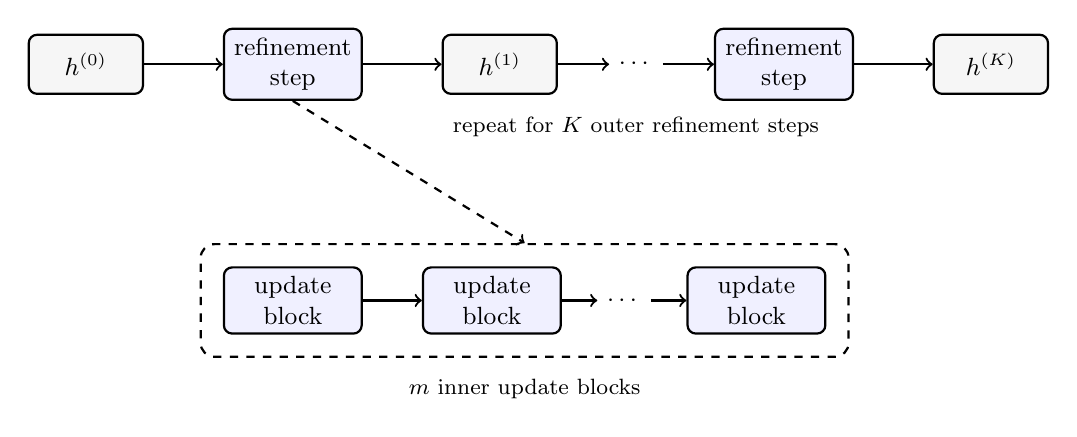
\begin{tikzpicture}[
    font=\small,
    block/.style={
        draw,
        rounded corners=3pt,
        thick,
        minimum width=1.45cm,
        minimum height=0.75cm,
        align=center,
        fill=gray!7
    },
    update/.style={
        draw,
        rounded corners=3pt,
        thick,
        minimum width=1.75cm,
        minimum height=0.72cm,
        align=center,
        fill=blue!6
    },
    arrow/.style={->, thick},
    note/.style={font=\footnotesize, align=center},
    outerbox/.style={
        draw,
        dashed,
        rounded corners=5pt,
        thick,
        inner sep=8pt
    }
]

\node[block] (h0) {$h^{(0)}$};

\node[update, right=1.0cm of h0] (step1) {refinement\\step};
\node[block, right=1.0cm of step1] (h1) {$h^{(1)}$};

\node[right=0.65cm of h1] (dots1) {$\cdots$};

\node[update, right=0.65cm of dots1] (stepk) {refinement\\step};
\node[block, right=1.0cm of stepk] (hk) {$h^{(K)}$};

\draw[arrow] (h0) -- (step1);
\draw[arrow] (step1) -- (h1);
\draw[arrow] (h1) -- (dots1);
\draw[arrow] (dots1) -- (stepk);
\draw[arrow] (stepk) -- (hk);

\node[note, below=0.35cm of dots1] {repeat for $K$ outer refinement steps};

\node[update, below=2.1cm of step1] (u1) {update\\block};
\node[update, right=0.75cm of u1] (u2) {update\\block};
\node[right=0.45cm of u2] (dots2) {$\cdots$};
\node[update, right=0.45cm of dots2] (um) {update\\block};

\draw[arrow] (u1) -- (u2);
\draw[arrow] (u2) -- (dots2);
\draw[arrow] (dots2) -- (um);

\node[outerbox, fit=(u1)(u2)(dots2)(um)] (innerbox) {};
\node[note, above=0.12cm of innerbox.north] {};

\node[note, below=0.15cm of innerbox.south] {$m$ inner update blocks};

\draw[arrow, dashed]
    (step1.south) -- node[right, note] {} (innerbox.north);

\end{tikzpicture}
}
\caption{
Overview of the recurrent refinement architecture.
Starting from an initial latent representation $h^{(0)}$, the model applies $K$ outer refinement steps.
Each refinement step consists of $m$ inner update blocks.
}
\label{fig:refinement-simple}
\end{figure}


\section{Related Work}
%4.29 这个是不是最好写成加粗短语+对应分段的形式 比如Offline goal-conditioned RL/iterative refinement/
Many areas of machine learning have recently explored architectures that allocate computation through repeated latent updates rather than a single feedforward pass. Universal Transformers apply recurrence over depth with shared transition functions and adaptive computation \citep{universal_transformer, act}, while Deep Equilibrium Models formulate prediction as convergence to an implicit fixed point \citep{deq}. A broader family of recurrent and iterative reasoning methods similarly performs multiple rounds of latent correction before producing a final prediction \citep{recurrent_relational_networks, energy_diffusion}. More recent systems such as HRM, TRM, and URM have renewed interest in this direction by showing that compact recurrent computation can be effective on supervised reasoning tasks \citep{hrm, trm, urm}. Reinforcement learning has also seen growing interest in architecture and scaling. Recent work has improved online RL agents by increasing network depth or width, adding residual structure, or otherwise strengthening feedforward actor-critic backbones \citep{thousand_layers, bro, simba}. These results suggest that value-function architecture can be an important factor in control performance. However, offline goal-conditioned RL poses a different scaling problem. In this setting, conventional feedforward architecture changes do not necessarily yield consistent gains, because the agent must infer goal reachability from a fixed dataset rather than repair value errors through additional interaction.

Offline goal-conditioned RL is particularly challenging because it combines long-horizon reasoning with the distributional constraints of offline learning. OGBench was introduced to study these difficulties through tasks that require stitching across trajectories, generalization over state-goal pairs, and robust policy extraction from learned value estimates \citep{ogbench}. Recent analyses further suggest that the main bottleneck in offline GCRL is not unique: value learning, policy extraction, and generalization can all limit performance depending on the algorithm and task \citep{ogbench, value_bottleneck}. 

Existing offline GCRL algorithms address these challenges from several directions. Contrastive RL learns a goal-conditioned compatibility score and trains the actor to optimize that score, providing a simple non-hierarchical actor-critic formulation \citep{crl, ogbench}. Hierarchical methods such as HIQL introduce temporal abstraction to improve long-horizon goal reaching \citep{hiql}. Other recent approaches, including SAW-style methods, focus on improving policy extraction or actor-side goal-conditioned learning under fixed datasets \citep{saw}. These directions are complementary to ours, as our work targets the value-learning side of this picture.




\section{Preliminaries}
\label{sec:preliminaries}
\paragraph{Offline goal-conditioned RL}
We consider an offline goal-conditioned Markov decision process with state space $\mathcal{S}$, action space $\mathcal{A}$, transition kernel $P$, and goal space $\mathcal{G}$. The learner is given a fixed dataset of trajectories $\mathcal{D}=\{\tau^{(n)}\}_{n=1}^{N}$, with $\tau=(s_0,a_0,s_1,\ldots,s_T)$, and receives no further environment interaction during training. Given an initial state and goal $g$, the objective is to learn a goal-conditioned policy $\pi(a\mid s,g)$ that maximizes the discounted goal-reaching return
\(
J(\pi)=
\mathbb{E}_{g \sim p(g),\, \tau \sim p^{\pi}(\tau \mid g)}
\left[
\sum_{t=0}^{\infty} \gamma^t r_g(s_t,a_t,s_{t+1})
\right],
\)
where $r_g$ is the sparse goal-reaching reward or its environment-specific analogue. During training, goals are sampled from the dataset, with future states providing positive reachability supervision and other dataset states providing contrastive comparisons.

\paragraph{Contrastive RL}
Contrastive RL (CRL) learns a goal-conditioned compatibility score and then extracts a policy from that score \citep{crl}. We write the critic as $f_{\phi,\psi}(s,a,g)$ and the actor as $\pi_\theta(a\mid s,g)$. CRL can be written as a binary-NCE objective that contrasts a future goal $g$ against a random goal $g^-$ \citep{ma_collins_binary_nce, crl}:
\begin{equation}
\mathcal{J}_{\mathrm{CRL}}(f)
=
\mathbb{E}_{(s,a)\sim p_{\mathcal{D}},\,g\sim p_{\mathcal{D}}^{\mathrm{future}}(\cdot\mid s,a),\,g^-\sim p_{\mathcal{D}}}
\left[
\log\sigma(f(s,a,g))+\log(1-\sigma(f(s,a,g^-)))
\right].
\end{equation}
In our experiments, the score is parameterized as a scaled inner product
\(f_{\phi,\psi}(s,a,g)=\phi(s,a)^\top\psi(g)/\sqrt{d}\).
For policy extraction, continuous-action CRL uses the DDPG+BC objective from OGBench, replacing $Q$ with the learned CRL score:
\begin{equation}
\mathcal{J}_{\mathrm{actor}}(\pi_\theta)
=
\mathbb{E}_{(s,a)\sim p_{\mathcal{D}},\,g\sim p_{\mathcal{D}}(\cdot\mid s)}
\left[
f_{\phi,\psi}(s,\pi_\theta^\mu(s,g),g)
+ \alpha \log \pi_\theta(a\mid s,g)
\right],
\end{equation}
where $\pi_\theta^\mu(s,g)$ is the mean action of the policy \citep{td3bc, ogbench}. Thus policy extraction depends directly on the learned score while remaining regularized toward behavior support. This direct score-to-actor interface is why CRL is our main diagnostic setting for studying how refinement changes value learning. We use the same CRL setup as OGBench to keep the comparison straightforward.

\paragraph{Iterative refinement}
Iterative refinement replaces a one-shot predictor with repeated latent updates. Given an input $x$, a recurrent-depth model initializes $h^{(0)}=\rho(x)$ and applies
\begin{equation}
h^{(k+1)}
=
h^{(k)} + F_{\theta}(h^{(k)}, x, e_k),
\qquad
k=0,\ldots,K-1,
\end{equation}
before predicting $\hat y = R(h^{(K)})$. The key feature is that the update parameters $\theta$ are tied across refinement steps, so depth is obtained by recurrently applying the same learned transformation rather than by stacking independent layers. This form of computation appears in Universal Transformers, adaptive computation methods, deep equilibrium models, and recurrent reasoning systems \citep{universal_transformer, act, deq, recurrent_relational_networks, energy_diffusion, hrm, trm, urm}. In practice, repeated updates are sensitive to optimization and scale. Step embeddings $e_k$ let a shared recurrent block distinguish refinement stages \citep{universal_transformer}, while normalization and residual scaling, such as LayerNorm and LayerScale, help stabilize deep or repeated computation \citep{layer_norm, layerscale}.
\section{Recurrent Latent Refinement}
\label{sec:architecture}

\begin{figure}[t]
\centering

% ============================================================
% Left panel: outer refinement step
% ============================================================
\begin{subfigure}[t]{0.48\linewidth}
\centering
\resizebox{\linewidth}{!}{
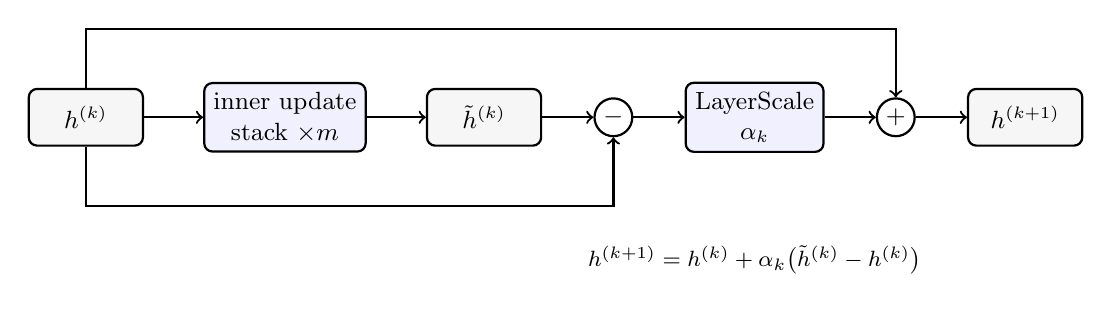
\begin{tikzpicture}[
    font=\small,
    block/.style={
        draw,
        rounded corners=3pt,
        thick,
        minimum width=1.45cm,
        minimum height=0.72cm,
        align=center,
        fill=gray!7
    },
    update/.style={
        draw,
        rounded corners=3pt,
        thick,
        minimum width=1.75cm,
        minimum height=0.72cm,
        align=center,
        fill=blue!6
    },
    op/.style={
        circle,
        draw,
        thick,
        minimum size=0.48cm,
        inner sep=0pt
    },
    arrow/.style={->, thick},
    note/.style={font=\footnotesize, align=center}
]

\node[block] (hk) {$h^{(k)}$};
\node[update, right=0.75cm of hk] (stack) {inner update\\stack $\times m$};
\node[block, right=0.75cm of stack] (htilde) {$\tilde h^{(k)}$};
\node[op, right=0.65cm of htilde] (minus) {$-$};
\node[update, right=0.65cm of minus] (scale) {LayerScale\\$\alpha_k$};
\node[op, right=0.65cm of scale] (plus) {$+$};
\node[block, right=0.65cm of plus] (hnext) {$h^{(k+1)}$};

% main straight path
\draw[arrow] (hk) -- (stack);
\draw[arrow] (stack) -- (htilde);
\draw[arrow] (htilde) -- (minus);
\draw[arrow] (minus) -- (scale);
\draw[arrow] (scale) -- (plus);
\draw[arrow] (plus) -- (hnext);

% straight right-angle branch to subtraction
\draw[arrow]
    (hk.south) -- ++(0,-0.75)
    -| (minus.south);

% straight right-angle residual branch to addition
\draw[arrow]
    (hk.north) -- ++(0,0.75)
    -| (plus.north);

\node[note, below=1.05cm of scale] 
{$h^{(k+1)} = h^{(k)} + \alpha_k\big(\tilde h^{(k)} - h^{(k)}\big)$};

\end{tikzpicture}
}
\caption{Outer refinement step.}
\label{fig:outer-refinement}
\end{subfigure}
\hfill
% ============================================================
% Right panel: inner update block
% ============================================================
\begin{subfigure}[t]{0.48\linewidth}
\centering
\resizebox{\linewidth}{!}{
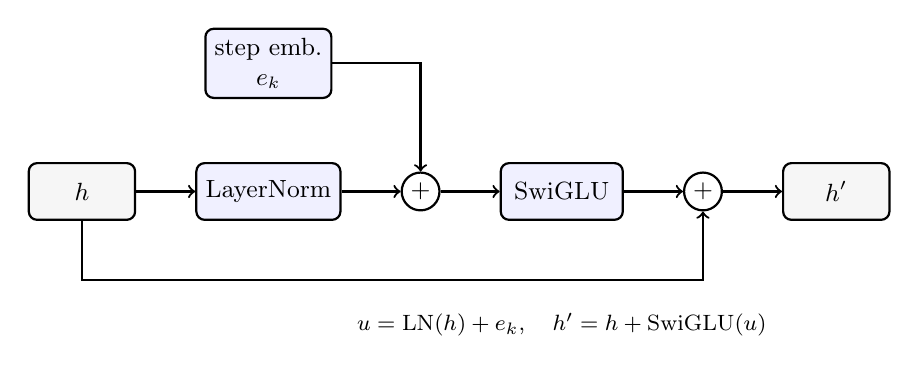
\begin{tikzpicture}[
    font=\small,
    block/.style={
        draw,
        rounded corners=3pt,
        thick,
        minimum width=1.35cm,
        minimum height=0.72cm,
        align=center,
        fill=gray!7
    },
    update/.style={
        draw,
        rounded corners=3pt,
        thick,
        minimum width=1.55cm,
        minimum height=0.72cm,
        align=center,
        fill=blue!6
    },
    op/.style={
        circle,
        draw,
        thick,
        minimum size=0.48cm,
        inner sep=0pt
    },
    arrow/.style={->, thick},
    note/.style={font=\footnotesize, align=center}
]

\node[block] (hin) {$h$};
\node[update, right=0.75cm of hin] (ln) {LayerNorm};
\node[update, above=0.8cm of ln] (step) {step emb.\\$e_k$};
\node[op, right=0.75cm of ln] (film) {$+$};
\node[update, right=0.75cm of film] (swiglu) {SwiGLU};
\node[op, right=0.75cm of swiglu] (plusres) {$+$};
\node[block, right=0.75cm of plusres] (hout) {$h'$};

% main path
\draw[arrow] (hin) -- (ln);
\draw[arrow] (ln) -- (film);
% Changed the -- to -| for the right-then-down routing
\draw[arrow] (step) -| (film); 
\draw[arrow] (film) -- (swiglu);
\draw[arrow] (swiglu) -- (plusres);
\draw[arrow] (plusres) -- (hout);

% straight residual branch
\draw[arrow]
    (hin.south) -- ++(0,-0.75)
    -| (plusres.south);

\node[note, below=1.05cm of swiglu]
{$u = \mathrm{LN}(h) + e_k,\quad h' = h + \mathrm{SwiGLU}(u)$};

\end{tikzpicture}
}
\caption{Inner update block.}
\label{fig:inner-update}
\end{subfigure}

\caption{
Architecture of the recurrent refinement module.
Left: the outer refinement step applies an inner update stack and uses LayerScale to control the refinement magnitude.
Right: each inner update block applies LayerNorm, step conditioning, SwiGLU transformation, and an inner residual update.
}
\label{fig:refinement-detailed}
\end{figure}

Figure~\ref{fig:refinement-detailed} illustrates the recurrent refinement block used as our value or critic backbone. We now specify the update shown in Figure~\ref{fig:refinement-detailed}. The module replaces a feedforward value or critic block while keeping the surrounding algorithm, losses, replay data, and optimization procedure unchanged. Given an input representation $x$, it initializes a latent state $h^{(0)}$ and refines it through $K$ outer iterations. Each outer iteration performs $m$ inner update blocks before exposing the next latent state, so $K$ controls how many times the representation is revised, while $m$ controls how expressive each revision is.

Each inner block uses pre-layer normalization, a learned outer-step embedding, a SwiGLU channel update, and residual computation \citep{layer_norm, universal_transformer, shazeer_glu}. Let $h^{(k,0)}=h^{(k)}$ denote the start of outer refinement step $k$. For inner block $j=1,\ldots,m$, we compute
\begin{equation}
h^{(k,j)}
=
h^{(k,j-1)}
+
W_{o,j}\,\mathrm{SwiGLU}_{j}
\!\left(\mathrm{LN}_{j}(h^{(k,j-1)}) + E_k\right),
\end{equation}
where $E_k$ is a learned embedding for the outer refinement step. The inner block weights are reused across outer iterations but are not tied across inner depth $j$, so increasing $m$ increases the capacity of a single refinement update without changing the number of outer revisions. After the $m$ inner updates, an outer LayerScale coefficient controls how much of the proposed update is accepted:
\begin{equation}
h^{(k+1)}
=
h^{(k)}
+
\alpha_k\left(h^{(k,m)}-h^{(k)}\right),
\qquad k=0,\ldots,K-1.
\end{equation}
Here $\alpha_k$ is initialized small and learned separately for each outer step, stabilizing repeated residual computation \citep{layerscale}. The case $m=1$ recovers a single-update refinement block, while $m>1$ gives a more expressive stacked-SwiGLU update within each refinement step. This design lets us vary repeated revision depth and per-step update capacity separately before the algorithm consumes the resulting value, score, or policy signal.



% \paragraph{Why recurrence helps}
% We do not attribute the advantage of the recurrent critic to increased
% expressivity, as an untied MLP can represent the unrolled computation
% \(Q \approx f_\theta(s,a,g)\). Instead, the difference is structural.
% In goal-conditioned RL, evaluating state-action--goal compatibility often
% requires implicit multi-step reasoning over the dataset, which can be
% viewed as approximating a compositional mapping \(Q^\star \approx T^K \circ \Phi\).
% A one-shot MLP must approximate this process in a single mapping, which
% entangles different stages of computation.

% In contrast, a recurrent critic performs iterative refinement
% \(h_{k+1} = h_k + F_\theta(h_k)\), and can be viewed as learning a local
% update rule that incrementally improves the representation. In this sense,
% it only needs to learn a direction of improvement that is locally correct
% (e.g., reducing a residual \(\|h_k - h^\star\|\)), while an MLP must
% represent a globally consistent mapping in one pass. When the target
% function admits a progressive refinement structure, such local updates can
% be substantially easier to learn than fitting \(f_\theta\) directly.
% This parameter sharing across steps therefore acts as a useful inductive
% bias, improving data efficiency and stability. This advantage is
% conditional and depends on the presence of such iterative structure.


\section{Experiments}
\subsection{Experiment Setup}\label{section:exp-setup}
\paragraph{Environments}
We evaluate on OGBench \citep{ogbench}, a benchmark designed specifically for offline goal-conditioned RL. In this setting the agent receives a fixed dataset of trajectories and must learn to reach new evaluation goals without any additional environment interaction. OGBench provides standardized datasets and multiple held-out state-goal evaluation pairs for each task, making it useful for testing long-horizon reachability, trajectory stitching, state-goal generalization, and policy extraction from offline data. The benchmark spans locomotion and manipulation domains: locomotion tasks require simulated agents to navigate mazes of different sizes and dataset types, while manipulation tasks require reaching object configurations or compositional scene goals. Following the benchmark protocol, we report average success over the five OGBench evaluation tasks for each dataset, with 50 episodes per task.


\paragraph{Algorithms and architecture}
We study recurrent latent refinement as an architecture-level replacement inside existing offline GCRL algorithms, rather than as a new loss or data-generation procedure. Our experiments include CRL, HIQL, and SAW as the main algorithmic settings. These methods expose different value-to-policy interfaces: CRL learns a contrastive state-action-goal score and extracts the actor with a DDPG+BC-style objective \citep{crl, td3bc}; HIQL uses hierarchical value learning with AWR-style actor extraction \citep{hiql}; and SAW uses a different policy-extraction procedure based on its own subgoal-weighted training objective \citep{saw}. In each comparison, the recurrent variant replaces the relevant MLP value or critic backbone with the tied refinement module from Section~\ref{sec:architecture}. The surrounding algorithm is otherwise held fixed, including the actor architecture, replay data, goal sampling, losses, batch size, optimizer, and evaluation protocol. Detailed HIQL and SAW insertion points, objectives, and hyperparameters are reported in the appendix.


\subsection{Main Results}\label{main-results}
The main recurrent-versus-MLP comparison across locomotion and manipulation datasets and across the evaluated offline GCRL algorithms is shown in Table~\ref{tab:main_results}. We use a unified row format so that each result keeps its algorithm, recurrent configuration, and dataset setting explicit.
\begin{table*}[h]
\centering
\scriptsize
\setlength{\tabcolsep}{4pt}
\begin{tabular}{lllccc}
\toprule
Algorithm & Recurrent config & Dataset group & MLP & Recurrent & $\Delta$ \\
\midrule
CRL  & $K=4,\,m=1$ & AMS & 0.530 & \textbf{0.954} & +0.424 \\
CRL  & $K=4,\,m=1$ & ALS & 0.110 & \textbf{0.479} & +0.369 \\
% CRL  & $K=4,\,m=1$ & ATS & 0.310 & \textbf{0.362} & +0.052 \\
CRL  & $K=4,\,m=1$ & AMN & 0.950 & \textbf{0.963} & +0.013 \\
CRL  & $K=4,\,m=1$ & ALN & 0.830 & \textbf{0.893} & +0.063 \\
CRL  & $K=4,\,m=1$ & AGN & 0.160 & \textbf{0.340} & +0.180 \\
% CRL  & $K=4,\,m=1$ & ATN & 0.200 & \textbf{0.557} & +0.357 \\
CRL  & $K=4,\,m=1$ & HMN & 0.600 & \textbf{0.632} & +0.032 \\
CRL  & $K=4,\,m=1$ & HMS & 0.360 & \textbf{0.657} & +0.297 \\
CRL  & $K=4,\,m=1$ & HLN &  &  &  \\
CRL  & $K=4,\,m=1$ & HLS &  &  &  \\
CRL  & $K=4,\,m=1$ & CSP & 0.100 & \textbf{0.205} & +0.105 \\
CRL  & $K=4,\,m=1$ & SP  & 0.190 & \textbf{0.288} & +0.110 \\
\midrule
HIQL & $K=4,\,m=2$ & AGN & 0.650 & \textbf{0.736} & +0.086 \\
HIQL & $K=4,\,m=2$ & ALS & 0.670 & \textbf{0.704} & +0.034 \\
% HIQL & $K=4,\,m=2$ & ATN & 0.420 & \textbf{0.468} & +0.048 \\
% HIQL & $K=4,\,m=2$ & ATS & 0.360 & \textbf{0.426} & +0.066 \\
HIQL & $K=4,\,m=2$ & HLN &  &  &  \\
HIQL & $K=4,\,m=2$ & HLS &  &  & \\
HIQL & $K=4,\,m=2$ & CSP & &  &  \\
HIQL & $K=4,\,m=2$ & SP & 0.38 & \textbf{0.572} &  \\
\midrule
SAW  & $K=4,\,m=1$ & AGN & 0.730 & \textbf{0.788} & +0.058 \\
SAW  & $K=4,\,m=1$ & HGN & 0.350 & \textbf{0.443} & +0.093 \\
SAW  & $K=4,\,m=1$ & CDP & 0.400 & \textbf{0.462} & +0.062 \\
SAW  & $K=4,\,m=1$ & SP  & 0.630 & \textbf{0.656} & +0.017 \\
\bottomrule
\end{tabular}
\caption{Main results in a unified row format. Each row reports average success rate across 8 seeds on one OGBench dataset setting for the MLP baseline and recurrent variant, with $\Delta$ denoting recurrent minus MLP.}
\label{tab:main_results}
\end{table*}


\subsection{Effect of Refinement Depth}
\label{sec:depth}
The main results use a fixed refinement depth, but the architecture is only meaningfully recurrent if repeated updates matter. We therefore sweep the number of outer refinement steps $K$ in CRL on \texttt{Antmaze-Medium-Stitch} (AMS) and \texttt{Antmaze-Giant-Navigate} (AGN), comparing the MLP baseline with $K\in\{1,2,4,6,8\}$ recurrent critics.

Figure~\ref{fig:iter_ams_agn} shows that a single refinement step does not explain the gain: $K=1$ remains close to the MLP baseline, while $K\geq2$ enters a substantially higher-success regime. Figure~\ref{fig:iter_1M_100k} summarizes the same pattern at early and final checkpoints. Performance is not a monotonic function of depth; it saturates after a small number of recurrent revisions and is strongest around $K=4$--$6$. We use $K=4$ as the default because it captures most of the gain while keeping computation moderate. Detailed numeric tables for the depth sweep are reported in the appendix.

\begin{figure}[h]
    \centering
    \includegraphics[width=\linewidth]{figures/iter_learning_process_steps.png}
    \caption{Learning curves for refinement-depth sweeps on AMS and AGN. Shaded regions indicate standard deviation over four seeds.}
    \label{fig:iter_ams_agn}
\end{figure}

\begin{figure}[h]
    \centering
    \includegraphics[width=\linewidth]{figures/iter_1M_100k.pdf}
    \caption{Success rates for MLP and $K$-step recurrent critics at early and final checkpoints on AMS and AGN, averaged over four seeds.}
    \label{fig:iter_1M_100k}
\end{figure}


\subsection{Effect of Per-Step Update Capacity}
The refinement module has two architectural axes: the number of outer refinement steps $K$ and the number of inner update blocks $m$ used within each step. After fixing $K=4$, we vary $m$ to test whether per-step update capacity matters. Table~\ref{tab:m_ablation} shows that it does, but not uniformly across algorithms. HIQL benefits from the more expressive $m=2$ update across ALS, AGN, and Scene, while CRL is stronger with $m=1$ on the AntMaze settings and roughly tied on Scene. Thus, $m$ is not a generic capacity knob; it interacts with the algorithmic value-to-policy interface. We use $m=1$ for CRL and $m=2$ for HIQL in the main comparisons.

\begin{table}[h]
\centering
\scriptsize
\setlength{\tabcolsep}{5pt}
\caption{Effect of inner update depth $m$ with $K=4$ fixed. Entries report average success with standard deviation.}
\label{tab:m_ablation}
\begin{tabular}{llcc}
\toprule
Dataset & Algorithm & $m=1$ & $m=2$ \\
\midrule
ALS & HIQL & 0.497 $\pm$ 0.043 & \textbf{0.691} $\pm$ 0.366 \\
ALS & CRL  & \textbf{0.504} $\pm$ 0.096 & 0.380 $\pm$ 0.153 \\
AGN & HIQL & 0.605 $\pm$ 0.056 & \textbf{0.722} $\pm$ 0.373 \\
AGN & CRL  & \textbf{0.331} $\pm$ 0.056 & 0.173 $\pm$ 0.083 \\
Scene & HIQL & 0.480 $\pm$ 0.028 & \textbf{0.565} $\pm$ 0.297 \\
Scene & CRL  & 0.288 $\pm$ 0.045 & \textbf{0.293} $\pm$ 0.135 \\
\bottomrule
\end{tabular}
\end{table}



\subsection{Why Is the Recurrent Critic Better?}\label{section:why better}
End-task success alone does not explain what recurrent refinement changes. We therefore use CRL as the main mechanism-analysis setting because its critic signal is exposed directly: CRL learns a compatibility score $f(s,a,g)$ and the DDPG+BC actor is trained to choose actions with high score under this critic. This lets us evaluate the learned signal at the policy-extraction interface, rather than only through final rollout success.

We focus on three state-based AntMaze tasks: \texttt{Antmaze-Medium-Stitch} (AMS), \texttt{Antmaze-Large-Stitch} (ALS), and \texttt{Antmaze-Giant-Navigate} (AGN). Unless stated otherwise, the comparison is between the default MLP CRL critic and the four-step recurrent CRL critic. The diagnostic tables report mean $\pm$ std over four MLP seeds for all tasks, four recurrent seeds for AMS, and three recurrent seeds for ALS and AGN.

We ask three diagnostic questions. First, does recurrence improve the critic's discrimination between reachable and sampled negative goals? Second, does the learned score induce a less extrapolative actor under offline policy extraction? Third, are the gains simply explained by better maze-distance prediction?

For critic discrimination, we use the contrastive structure of CRL. A dataset transition paired with a future goal from the same trajectory is treated as a positive pair, while pairing the same transition with a sampled goal gives a negative pair. Let $q^+=f(s,a,g)$ and $q^-=f(s,a,g^-)$ denote these matched and mismatched scores. We report the raw margin $\mathbb{E}[q^+-q^-]$, ranking accuracy $\Pr[q^+>q^-]$, and normalized separation
\[
\mathrm{Sep}
=
\frac{\mathbb{E}[q^+-q^-]}{\sqrt{\mathrm{Var}(q^+) + \mathrm{Var}(q^-) + \epsilon}}.
\]
For actor-interface diagnostics, we compare the critic scores of the extracted actor action and the dataset action on the same state-goal pairs:
\[
q_\Delta
=
\mathbb{E}_{(s,a_{\mathcal D},g)}
\left[
f(s,\pi^\mu(s,g),g)-f(s,a_{\mathcal D},g)
\right].
\]
We also report the fraction of pairs where the critic prefers the actor action, policy--behavior MSE/L2 distance, and the actor log probability of the dataset action, $\mathbb{E}[\log \pi(a_{\mathcal D}\mid s,g)]$. Lower $q_\Delta$ and smaller policy--behavior distance indicate less extrapolative actor extraction. Finally, graph-distance correlations test whether recurrence is merely learning a better shortest-path surrogate.

\paragraph{Critic discrimination improves in normalized form.}
Across AMS, ALS, and AGN, recurrent refinement improves normalized separation between matched and mismatched goals (Figure~\ref{fig:success_sep_graphcorr}(a,b); full statistics in Table~\ref{tab:critic_diagnostics_app}). This should not be interpreted as a uniform increase in raw margin. On AMS, the recurrent critic increases the raw margin; on ALS and AGN, the raw margin decreases, while the score variability also decreases enough that normalized separation still improves. The critic-side effect is therefore more specific than score scaling: recurrence changes the distribution of scores in a way that improves normalized positive-negative discrimination.

\begin{figure}[h]
    \centering
    \includegraphics[width=\linewidth]{figures/success_sep_graphcorr_full.pdf}
    \caption{Mechanism summary of recurrent critic improvements across AMS, ALS, and AGN.}
    \label{fig:success_sep_graphcorr}
\end{figure}

\paragraph{Actor extraction becomes less extrapolative.}
The clearest diagnostic change appears at the actor interface. With the recurrent critic, the extracted actor reaches higher success while staying closer to dataset actions. Across AMS, ALS, and AGN, $q_\Delta$ decreases, policy MSE and L2 distance decrease, and the actor assigns higher log probability to dataset actions (Table~\ref{tab:actor_diagnostics_app}). These trends are consistent with the recurrent critic providing a more usable offline policy-extraction signal: the actor can improve goal-reaching performance without relying as strongly on critic-preferred actions far from the dataset.

\begin{figure}[h]
    \centering
    \begin{subfigure}[b]{0.48\textwidth}
        \includegraphics[width=\linewidth]{figures/mse.pdf}
        \caption{Policy MSE}
        \label{fig:mse}
    \end{subfigure}
    \hfill
    \begin{subfigure}[b]{0.48\textwidth}
        \includegraphics[width=\linewidth]{figures/qdelta.pdf}
        \caption{$q_\Delta$}
        \label{fig:qdelta}
    \end{subfigure}
    \caption{Actor-interface diagnostics. Recurrent refinement improves success while reducing policy deviation from dataset actions and reducing the actor-over-dataset critic gap.}
    \label{fig:mse+qdelta}
\end{figure}

\paragraph{Trajectory effects appear at bottlenecks.}
The task-wise results show that the aggregate gains are heterogeneous across goals (Table~\ref{tab:taskwise_success_app}). On AMS, recurrence improves all five goals, with especially large gains on tasks where the MLP actor often fails. ALS shows gains across several subtasks, although one task remains unsolved by both methods. AGN remains the hardest diagnostic setting, but recurrent refinement still improves average success and several individual goals. This pattern is consistent with an environment-level interpretation: in maze layouts, the actor often needs to choose behavior-like actions that are not locally goal-directed, such as entering a corridor, completing a turn, or temporarily moving away from the goal to follow a U-shaped path.

\begin{figure}[t]
    \centering
    \includegraphics[width=\linewidth]{figures/ams_trajectory_bottleneck.pdf}
    \caption{Trajectory-level visualization of actor extraction on AMS bottleneck tasks. For each task, the left panel shows the maze layout with start and goal, while the middle and right panels show matched-seed trajectories from the MLP baseline and recurrent critic.}
    \label{fig:ams_trajectory_bottleneck}
\end{figure}

The trajectory visualization in Figure~\ref{fig:ams_trajectory_bottleneck} makes this actor-interface effect concrete. The MLP actor can reach a bottleneck region but stall or follow a locally tempting direction, while the recurrent-critic actor follows the corridor structure more reliably. This qualitative behavior matches the quantitative diagnostics: recurrent refinement keeps the actor closer to dataset behavior while making behavior-like actions more useful for long-horizon navigation.

\paragraph{Not merely better graph-distance prediction.}
Finally, graph-distance correlations argue against a simpler explanation. If recurrence merely learned a better shortest-path heuristic, graph correlations should improve consistently. Instead, control improves on AMS and ALS while graph-distance correlations decrease or remain mixed, and AGN is mixed across correlation metrics (Table~\ref{tab:graph_corr_app}). Thus the diagnostics are most consistent with recurrence improving the actor-facing value signal, rather than simply producing a uniformly better graph-distance estimator.

\iffalse


\fi

\subsection{Matched Parameter and Computation Comparison}\label{matched}
A natural alternative explanation is that the recurrent critic improves only because it has more parameters than the default CRL critic. We test this with dense feedforward controls that keep the same MLP recipe as CRL's critic, including GELU activations and layer normalization, but match the recurrent critic's parameter count by either increasing depth or increasing width.
\begin{figure}[h]
    \centering
    \includegraphics[width=\linewidth]{figures/parameter_match.pdf}
    \caption{Matched-parameter dense feedforward controls. The recurrent critic is compared with depth-matched and width-matched dense MLP critics.}
    \label{fig:parameter_match}
\end{figure}
The two dense alternatives are a wider critic with hidden sizes \texttt{688-688-688} and a deeper critic with hidden sizes \texttt{512-512-512-512-512}, within 0.37\% and 0.19\% of the recurrent critic's parameter count, respectively. As shown in Figure~\ref{fig:parameter_match}, neither dense alternative closes the gap to the recurrent critic. This suggests that the improvement is not explained by parameter count alone, but by how the critic reuses computation through iterative latent refinement.


\subsection{Ablation on Model Components}
We next isolate the components of the recurrent update while keeping the CRL algorithm and four refinement steps fixed. The dense feedforward controls above remove iterative refinement entirely; here, each variant retains recurrence but removes one stabilizing or conditioning mechanism: step embeddings, pre-normalization in the update block, or LayerScale on the residual update.
\begin{figure}[h]
    \centering
    \includegraphics[width=\linewidth]{figures/ablation.pdf}
    \caption{Component ablations for the recurrent CRL critic on \texttt{Antmaze-Medium-Stitch} and \texttt{Antmaze-Large-Stitch}.}
    \label{fig:ablation}
\end{figure}
Figure~\ref{fig:ablation} shows that the full design is consistently strongest on both tasks. Removing LayerScale causes the largest drop, especially on \texttt{Antmaze-Large-Stitch}, supporting its role in controlling the scale of repeated residual updates. Removing pre-normalization also reduces performance, while removing step embeddings has a smaller effect on saturated success rates. The appendix diagnostics show that step conditioning still improves the learned representation: even when success remains high, margins and trajectory-consistency scores decrease without step information (Table~\ref{tab:component_ablation_app}).

Overall, the ablations support a structured design rather than recurrence alone: dense parameter-matched critics do not recover the same performance, and the recurrent critic is most reliable when residual refinement is normalized, scaled, and conditioned on the refinement step.


\section{Conclusion}
Reinforcement learning has often relied on comparatively shallow value and policy networks, and recent work has begun to challenge this convention by scaling depth, width, and regularization in RL architectures \citep{thousand_layers, bro, simba}. Our results suggest a complementary way to allocate computation: rather than only making the feedforward critic larger, offline GCRL can benefit from recurrently refining the value representation before policy extraction. This connects value learning to recurrent-depth and iterative reasoning models, where repeated latent updates support structured inference \citep{universal_transformer, deq, recurrent_relational_networks, energy_diffusion, hrm, trm, urm}. In offline GCRL, the critic must infer long-horizon reachability from fixed data and provide an actor-usable signal \citep{ogbench, value_bottleneck}; recurrent refinement improves this interface by producing a more discriminative and actor-friendly signal, especially on stitching and bottleneck tasks. Because the same architectural principle improves algorithms with different training regimes without changing their objectives or data, we view iterative refinement as a practical design axis for offline RL that complements losses, datasets, and policy-extraction methods.


\paragraph{Limitations.}
Our study is empirical and focused on offline GCRL, primarily on OGBench. Because recurrent variants are more expensive to train than single-pass critics, we do not exhaustively cover all datasets, algorithms, and hyperparameter regimes. The best recurrent configuration is also not universal: refinement depth $K$ and inner update capacity $m$ interact with the algorithm and environment, so recurrent computation must be allocated deliberately rather than scaled blindly. A useful next step is to develop selection rules that predict a good balance between outer refinement depth and per-step update capacity before training. Adaptive computation is another natural direction, but applying mechanisms such as ACT \citep{act} to GCRL is nontrivial because there is no direct per-example halting signal during value learning. Finally, our mechanism analysis is diagnostic rather than causal, and the present experiments leave open the boundary of where iterative refinement helps. Future work should test broader offline and online RL settings, combine recurrent refinement with complementary algorithmic improvements, and develop a more principled account of when allocating computation through iterative value refinement is most beneficial.






% \section{Submission of papers to NeurIPS 2026}


% Please read the instructions below carefully and follow them faithfully.


% \subsection{Style}


% Papers to be submitted to NeurIPS 2026 must be prepared according to the
% instructions presented here. Papers may only be up to {\bf nine} pages long, including figures. \textbf{Papers that exceed the page limit will not be reviewed (or in any other way considered) for presentation at the conference.}
% Additional pages \emph{containing acknowledgments, references, checklist, and optional technical appendices} do not count as content pages. 


% The margins in 2026 are the same as those in previous years.


% Authors are required to use the NeurIPS \LaTeX{} style files obtainable at the NeurIPS website as indicated below. Please make sure you use the current files and not previous versions. Tweaking the style files may be grounds for desk rejection.


% \subsection{Retrieval of style files}


% The style files for NeurIPS and other conference information are available on the website at
% \begin{center}
%   \url{https://neurips.cc}.
% \end{center}
% % The file \verb+neurips_2026.pdf+ contains these instructions and illustrates the various formatting requirements your NeurIPS paper must satisfy.


% The only supported style file for NeurIPS 2026 is \verb+neurips_2026.sty+, rewritten for \LaTeXe{}. \textbf{Previous style files for \LaTeX{} 2.09,  Microsoft Word, and RTF are no longer supported.}


% The \LaTeX{} style file contains three optional arguments: 
% \begin{itemize}
% \item \verb+final+, which creates a camera-ready copy, 
% \item \verb+preprint+, which creates a preprint for submission to, e.g., arXiv, \item \verb+nonatbib+, which will not load the \verb+natbib+ package for you in case of package clash.
% \end{itemize}


% \paragraph{Preprint option}
% If you wish to post a preprint of your work online, e.g., on arXiv, using the NeurIPS style, please use the \verb+preprint+ option. This will create a nonanonymized version of your work with the text ``Preprint. Work in progress.'' in the footer. This version may be distributed as you see fit, as long as you do not say which conference it was submitted to. Please \textbf{do not} use the \verb+final+ option, which should \textbf{only} be used for papers accepted to NeurIPS.


% At submission time, please omit the \verb+final+ and \verb+preprint+ options. This will anonymize your submission and add line numbers to aid review. Please do \emph{not} refer to these line numbers in your paper as they will be removed during generation of camera-ready copies.


% The file \verb+neurips_2026.tex+ may be used as a ``shell'' for writing your paper. All you have to do is replace the author, title, abstract, and text of the paper with your own.


% The formatting instructions contained in these style files are summarized in Sections \ref{gen_inst}, \ref{headings}, and \ref{others} below.


% \section{General formatting instructions}
% \label{gen_inst}


% The text must be confined within a rectangle 5.5~inches (33~picas) wide and
% 9~inches (54~picas) long. The left margin is 1.5~inch (9~picas).  Use 10~point
% type with a vertical spacing (leading) of 11~points.  Times New Roman is the
% preferred typeface throughout, and will be selected for you by default.
% Paragraphs are separated by \nicefrac{1}{2}~line space (5.5 points), with no
% indentation.


% The paper title should be 17~point, initial caps/lower case, bold, centered
% between two horizontal rules. The top rule should be 4~points thick and the
% bottom rule should be 1~point thick. Allow \nicefrac{1}{4}~inch space above and
% below the title to rules. All pages should start at 1~inch (6~picas) from the
% top of the page.


% For the final version, authors' names are set in boldface, and each name is
% centered above the corresponding address. The lead author's name is to be listed
% first (left-most), and the co-authors' names (if different address) are set to
% follow. If there is only one co-author, list both author and co-author side by
% side.


% Please pay special attention to the instructions in Section \ref{others}
% regarding figures, tables, acknowledgments, and references.

% \section{Headings: first level}
% \label{headings}


% All headings should be lower case (except for first word and proper nouns),
% flush left, and bold.


% First-level headings should be in 12-point type.


% \subsection{Headings: second level}


% Second-level headings should be in 10-point type.


% \subsubsection{Headings: third level}


% Third-level headings should be in 10-point type.


% \paragraph{Paragraphs}


% There is also a \verb+\paragraph+ command available, which sets the heading in
% bold, flush left, and inline with the text, with the heading followed by 1\,em
% of space.


% \section{Citations, figures, tables, references}
% \label{others}


% These instructions apply to everyone.


% \subsection{Citations within the text}


% The \verb+natbib+ package will be loaded for you by default.  Citations may be
% author/year or numeric, as long as you maintain internal consistency.  As to the
% format of the references themselves, any style is acceptable as long as it is
% used consistently.


% The documentation for \verb+natbib+ may be found at
% \begin{center}
%   \url{http://mirrors.ctan.org/macros/latex/contrib/natbib/natnotes.pdf}
% \end{center}
% Of note is the command \verb+\citet+, which produces citations appropriate for
% use in inline text.  For example,
% \begin{verbatim}
%    \citet{hasselmo} investigated\dots
% \end{verbatim}
% produces
% \begin{quote}
%   Hasselmo, et al.\ (1995) investigated\dots
% \end{quote}


% If you wish to load the \verb+natbib+ package with options, you may add the
% following before loading the \verb+neurips_2026+ package:
% \begin{verbatim}
%    \PassOptionsToPackage{options}{natbib}
% \end{verbatim}


% If \verb+natbib+ clashes with another package you load, you can add the optional
% argument \verb+nonatbib+ when loading the style file:
% \begin{verbatim}
%    \usepackage[nonatbib]{neurips_2026}
% \end{verbatim}


% As submission is double blind, refer to your own published work in the third
% person. That is, use ``In the previous work of Jones et al.\ [4],'' not ``In our
% previous work [4].'' If you cite your other papers that are not widely available
% (e.g., a journal paper under review), use anonymous author names in the
% citation, e.g., an author of the form ``A.\ Anonymous'' and include a copy of the anonymized paper in the supplementary material.


% \subsection{Footnotes}


% Footnotes should be used sparingly.  If you do require a footnote, indicate
% footnotes with a number\footnote{Sample of the first footnote.} in the
% text. Place the footnotes at the bottom of the page on which they appear.
% Precede the footnote with a horizontal rule of 2~inches (12~picas).


% Note that footnotes are properly typeset \emph{after} punctuation
% marks.\footnote{As in this example.}


% \subsection{Figures}


% \begin{figure}
%   \centering
%   \fbox{\rule[-.5cm]{0cm}{4cm} \rule[-.5cm]{4cm}{0cm}}
%   \caption{Sample figure caption. Explain what the figure shows and add a key take-away message to the caption.}
% \end{figure}


% All artwork must be neat, clean, and legible. Lines should be dark enough for
%  reproduction purposes. The figure number and caption always appear after the
% figure. Place one line space before the figure caption and one line space after
% the figure. The figure caption should be lower case (except for the first word and proper nouns); figures are numbered consecutively.


% You may use color figures.  However, it is best for the figure captions and the
% paper body to be legible if the paper is printed in either black/white or in
% color.


% \subsection{Tables}


% All tables must be centered, neat, clean, and legible.  The table number and
% title always appear before the table.  See Table~\ref{sample-table}.


% Place one line space before the table title, one line space after the
% table title, and one line space after the table. The table title must
% be lower case (except for the first word and proper nouns); tables are
% numbered consecutively.


% Note that publication-quality tables \emph{do not contain vertical rules}. We
% strongly suggest the use of the \verb+booktabs+ package, which allows for
% typesetting high-quality, professional tables:
% \begin{center}
%   \url{https://www.ctan.org/pkg/booktabs}
% \end{center}
% This package was used to typeset Table~\ref{sample-table}.


% \begin{table}
%   \caption{Sample table caption. Explain what the table shows and add a key take-away message to the caption.}
%   \label{sample-table}
%   \centering
%   \begin{tabular}{lll}
%     \toprule
%     \multicolumn{2}{c}{Part}                   \\
%     \cmidrule(r){1-2}
%     Name     & Description     & Size ($\mu$m) \\
%     \midrule
%     Dendrite & Input terminal  & $\approx$100     \\
%     Axon     & Output terminal & $\approx$10      \\
%     Soma     & Cell body       & up to $10^6$  \\
%     \bottomrule
%   \end{tabular}
% \end{table}

% \subsection{Math}
% Note that display math in bare TeX commands will not create correct line numbers for submission. Please use LaTeX (or AMSTeX) commands for unnumbered display math. (You really shouldn't be using \$\$ anyway; see \url{https://tex.stackexchange.com/questions/503/why-is-preferable-to} and \url{https://tex.stackexchange.com/questions/40492/what-are-the-differences-between-align-equation-and-displaymath} for more information.)

% \subsection{Final instructions}

% Do not change any aspects of the formatting parameters in the style files.  In
% particular, do not modify the width or length of the rectangle the text should
% fit into, and do not change font sizes. Please note that pages should be
% numbered.


% \section{Preparing PDF files}


% Please prepare submission files with paper size ``US Letter,'' and not, for
% example, ``A4.''


% Fonts were the main cause of problems in the past years. Your PDF file must only
% contain Type 1 or Embedded TrueType fonts. Here are a few instructions to
% achieve this.


% \begin{itemize}


% \item You should directly generate PDF files using \verb+pdflatex+.


% \item You can check which fonts a PDF files uses.  In Acrobat Reader, select the
%   menu Files$>$Document Properties$>$Fonts and select Show All Fonts. You can
%   also use the program \verb+pdffonts+ which comes with \verb+xpdf+ and is
%   available out-of-the-box on most Linux machines.


% \item \verb+xfig+ ``patterned'' shapes are implemented with bitmap fonts.  Use
%   "solid" shapes instead.


% \item The \verb+\bbold+ package almost always uses bitmap fonts.  You should use
%   the equivalent AMS Fonts:
% \begin{verbatim}
%    \usepackage{amsfonts}
% \end{verbatim}
% followed by, e.g., \verb+\mathbb{R}+, \verb+\mathbb{N}+, or \verb+\mathbb{C}+
% for $\mathbb{R}$, $\mathbb{N}$ or $\mathbb{C}$.  You can also use the following
% workaround for reals, natural and complex:
% \begin{verbatim}
%    \newcommand{\RR}{I\!\!R} %real numbers
%    \newcommand{\Nat}{I\!\!N} %natural numbers
%    \newcommand{\CC}{I\!\!\!\!C} %complex numbers
% \end{verbatim}
% Note that \verb+amsfonts+ is automatically loaded by the \verb+amssymb+ package.


% \end{itemize}


% If your file contains type 3 fonts or non embedded TrueType fonts, we will ask
% you to fix it.


% \subsection{Margins in \LaTeX{}}


% Most of the margin problems come from figures positioned by hand using
% \verb+\special+ or other commands. We suggest using the command
% \verb+\includegraphics+ from the \verb+graphicx+ package. Always specify the
% figure width as a multiple of the line width as in the example below:
% \begin{verbatim}
%    \usepackage[pdftex]{graphicx} ...
%    \includegraphics[width=0.8\linewidth]{myfile.pdf}
% \end{verbatim}
% See Section 4.4 in the graphics bundle documentation
% (\url{http://mirrors.ctan.org/macros/latex/required/graphics/grfguide.pdf})


% A number of width problems arise when \LaTeX{} cannot properly hyphenate a
% line. Please give LaTeX hyphenation hints using the \verb+\-+ command when
% necessary.

% \begin{ack}
% Use unnumbered first level headings for the acknowledgments. All acknowledgments
% go at the end of the paper before the list of references. Moreover, you are required to declare
% funding (financial activities supporting the submitted work) and competing interests (related financial activities outside the submitted work).
% More information about this disclosure can be found at: \url{https://neurips.cc/Conferences/2026/PaperInformation/FundingDisclosure}.


% Do {\bf not} include this section in the anonymized submission, only in the final paper. You can use the \texttt{ack} environment provided in the style file to automatically hide this section in the anonymized submission.
% \end{ack}

\bibliographystyle{plainnat}
\nocite{*}
\bibliography{references}

%%%%%%%%%%%%%%%%%%%%%%%%%%%%%%%%%%%%%%%%%%%%%%%%%%%%%%%%%%%%

\appendix

\section{Depth Sweep Tables}
\begin{table}[h]
\centering
\scriptsize
\setlength{\tabcolsep}{2.5pt}
\caption{Final-checkpoint refinement-depth sweep on AMS. Metrics report mean $\pm$ std over four seeds.}
\label{tab:depth_final_app}
\resizebox{\linewidth}{!}{%
\begin{tabular}{lcccccccc}
\toprule
Setting & Final success$\uparrow$ & Best success$\uparrow$ & Best step & Margin & Rank & Sep. $z$ & Long margin & Long rank \\
\midrule
MLP & 0.506 $\pm$ 0.101 & 0.574 $\pm$ 0.063 & 450k $\pm$ 173k & 23.644 $\pm$ 0.931 & 0.990 $\pm$ 0.002 & 1.731 $\pm$ 0.027 & 22.625 $\pm$ 0.718 & 0.987 $\pm$ 0.003 \\
\texttt{iter1} & 0.638 $\pm$ 0.062 & 0.697 $\pm$ 0.040 & 725k $\pm$ 189k & 21.111 $\pm$ 0.571 & 0.992 $\pm$ 0.003 & 2.049 $\pm$ 0.034 & 20.251 $\pm$ 0.453 & 0.989 $\pm$ 0.004 \\
\texttt{iter2} & 0.914 $\pm$ 0.036 & 0.936 $\pm$ 0.018 & 750k $\pm$ 265k & 28.754 $\pm$ 1.049 & 0.996 $\pm$ 0.001 & 2.080 $\pm$ 0.041 & 27.687 $\pm$ 0.714 & 0.994 $\pm$ 0.002 \\
\texttt{iter4} & 0.947 $\pm$ 0.015 & \textbf{0.961} $\pm$ 0.020 & 850k $\pm$ 173k & 27.644 $\pm$ 0.564 & 0.998 $\pm$ 0.002 & 2.109 $\pm$ 0.055 & 27.005 $\pm$ 0.445 & 0.997 $\pm$ 0.002 \\
\texttt{iter6} & \textbf{0.956} $\pm$ 0.011 & 0.960 $\pm$ 0.004 & 950k $\pm$ 100k & 27.983 $\pm$ 0.623 & 0.998 $\pm$ 0.001 & 2.135 $\pm$ 0.034 & 27.236 $\pm$ 0.450 & 0.997 $\pm$ 0.002 \\
\texttt{iter8} & 0.912 $\pm$ 0.034 & 0.948 $\pm$ 0.041 & 825k $\pm$ 96k & 28.465 $\pm$ 0.679 & 0.999 $\pm$ 0.001 & 2.189 $\pm$ 0.059 & 27.896 $\pm$ 0.473 & 0.998 $\pm$ 0.001 \\
\bottomrule
\end{tabular}
}
\end{table}

\begin{table}[h]
\centering
\scriptsize
\setlength{\tabcolsep}{3pt}
\caption{Early-stage AMS refinement-depth sweep at 100k training steps. Metrics report mean $\pm$ std over four seeds.}
\label{tab:depth_early_app}
\begin{tabular}{lccccc}
\toprule
Setting & 100k success$\uparrow$ & Margin & Rank & Sep. $z$ & Long rank \\
\midrule
MLP & 0.377 $\pm$ 0.067 & 12.786 $\pm$ 0.134 & 0.985 $\pm$ 0.002 & 2.273 $\pm$ 0.056 & 0.980 $\pm$ 0.003 \\
\texttt{iter1} & 0.380 $\pm$ 0.140 & 10.611 $\pm$ 0.171 & 0.977 $\pm$ 0.005 & 2.255 $\pm$ 0.035 & 0.970 $\pm$ 0.005 \\
\texttt{iter2} & 0.609 $\pm$ 0.018 & 12.070 $\pm$ 0.158 & 0.987 $\pm$ 0.004 & 2.389 $\pm$ 0.056 & 0.984 $\pm$ 0.005 \\
\texttt{iter4} & 0.680 $\pm$ 0.027 & 12.995 $\pm$ 0.423 & 0.988 $\pm$ 0.004 & 2.419 $\pm$ 0.096 & 0.983 $\pm$ 0.006 \\
\texttt{iter6} & 0.731 $\pm$ 0.043 & 13.260 $\pm$ 0.152 & 0.988 $\pm$ 0.002 & 2.480 $\pm$ 0.086 & 0.984 $\pm$ 0.003 \\
\texttt{iter8} & \textbf{0.727} $\pm$ 0.076 & 13.517 $\pm$ 0.329 & 0.990 $\pm$ 0.003 & 2.491 $\pm$ 0.098 & 0.987 $\pm$ 0.005 \\
\bottomrule
\end{tabular}
\end{table}

\section{Additional Diagnostic Tables}

\begin{table}[h]
\centering
\scriptsize
\setlength{\tabcolsep}{2.5pt}
\caption{Critic discrimination diagnostics for the MLP and recurrent CRL critics. Success reports best evaluation success; other metrics are measured from the final diagnostic logs.}
\label{tab:critic_diagnostics_app}
\resizebox{\linewidth}{!}{%
\begin{tabular}{lcccccc}
\toprule
Metric & AMS+MLP & AMS+Ours & ALS+MLP & ALS+Ours & AGN+MLP & AGN+Ours \\
\midrule
Best success$\uparrow$ & 0.574 $\pm$ 0.063 & \textbf{0.953} $\pm$ 0.020 & 0.193 $\pm$ 0.020 & \textbf{0.455} $\pm$ 0.014 & 0.161 $\pm$ 0.023 & \textbf{0.373} $\pm$ 0.037 \\
Pos. mean & -2.490 $\pm$ 0.069 & -1.396 $\pm$ 0.124 & -2.080 $\pm$ 0.045 & -2.043 $\pm$ 0.018 & -3.421 $\pm$ 0.079 & -3.425 $\pm$ 0.112 \\
Neg. mean & -26.133 $\pm$ 0.866 & -29.040 $\pm$ 0.451 & -27.875 $\pm$ 0.187 & -23.225 $\pm$ 0.160 & -16.586 $\pm$ 0.391 & -15.183 $\pm$ 0.288 \\
Margin & 23.644 $\pm$ 0.931 & 27.644 $\pm$ 0.564 & 25.795 $\pm$ 0.221 & 21.183 $\pm$ 0.158 & 13.165 $\pm$ 0.468 & 11.759 $\pm$ 0.400 \\
Margin std. & 14.039 $\pm$ 0.500 & 13.351 $\pm$ 0.225 & 11.734 $\pm$ 0.202 & 8.765 $\pm$ 0.301 & 9.766 $\pm$ 0.238 & 8.082 $\pm$ 0.212 \\
Rank acc. & 0.990 $\pm$ 0.002 & 0.998 $\pm$ 0.002 & 0.995 $\pm$ 0.002 & 0.997 $\pm$ 0.002 & 0.973 $\pm$ 0.002 & 0.974 $\pm$ 0.001 \\
Separation $z$ & 1.731 $\pm$ 0.027 & 2.109 $\pm$ 0.055 & 2.231 $\pm$ 0.040 & 2.487 $\pm$ 0.048 & 1.474 $\pm$ 0.020 & 1.609 $\pm$ 0.048 \\
\bottomrule
\end{tabular}
}
\end{table}

\begin{table}[h]
\centering
\scriptsize
\setlength{\tabcolsep}{2.5pt}
\caption{Actor-interface diagnostics for the MLP and recurrent CRL critics. Lower $q_\Delta$ and lower policy deviation indicate less extrapolative policy extraction; higher behavior log probability means the actor assigns higher likelihood to dataset actions.}
\label{tab:actor_diagnostics_app}
\resizebox{\linewidth}{!}{%
\begin{tabular}{lcccccc}
\toprule
Metric & AMS+MLP & AMS+Ours & ALS+MLP & ALS+Ours & AGN+MLP & AGN+Ours \\
\midrule
$q_{\mathrm{actor}}$ & -10.798 $\pm$ 0.462 & -12.385 $\pm$ 0.534 & -12.092 $\pm$ 0.367 & -11.242 $\pm$ 0.251 & -5.134 $\pm$ 0.063 & -5.148 $\pm$ 0.038 \\
$q_{\mathrm{behavior}}$ & -11.642 $\pm$ 0.459 & -12.650 $\pm$ 0.525 & -12.598 $\pm$ 0.404 & -11.568 $\pm$ 0.273 & -5.337 $\pm$ 0.063 & -5.275 $\pm$ 0.048 \\
$q_{\Delta}\downarrow$ & 0.844 $\pm$ 0.035 & \textbf{0.265} $\pm$ 0.049 & 0.506 $\pm$ 0.056 & \textbf{0.326} $\pm$ 0.030 & 0.203 $\pm$ 0.010 & \textbf{0.127} $\pm$ 0.013 \\
Prefer actor & 0.701 $\pm$ 0.005 & 0.557 $\pm$ 0.017 & 0.681 $\pm$ 0.015 & 0.662 $\pm$ 0.013 & 0.697 $\pm$ 0.010 & 0.678 $\pm$ 0.011 \\
Policy MSE$\downarrow$ & 0.137 $\pm$ 0.005 & \textbf{0.082} $\pm$ 0.001 & 0.106 $\pm$ 0.006 & \textbf{0.087} $\pm$ 0.003 & 0.084 $\pm$ 0.004 & \textbf{0.067} $\pm$ 0.005 \\
Policy L2$\downarrow$ & 0.907 $\pm$ 0.015 & \textbf{0.734} $\pm$ 0.004 & 0.821 $\pm$ 0.015 & \textbf{0.752} $\pm$ 0.013 & 0.751 $\pm$ 0.016 & \textbf{0.683} $\pm$ 0.021 \\
Behavior log prob.$\uparrow$ & -7.899 $\pm$ 0.020 & \textbf{-7.680} $\pm$ 0.005 & -7.776 $\pm$ 0.023 & \textbf{-7.698} $\pm$ 0.014 & -7.688 $\pm$ 0.018 & \textbf{-7.621} $\pm$ 0.019 \\
\bottomrule
\end{tabular}
}
\end{table}

\begin{table}[h]
\centering
\scriptsize
\setlength{\tabcolsep}{2.5pt}
\caption{Task-wise final evaluation success. The gains are heterogeneous across goals, motivating trajectory-level visualization rather than a claim that a single scalar critic statistic explains every task.}
\label{tab:taskwise_success_app}
\resizebox{\linewidth}{!}{%
\begin{tabular}{lcccccc}
\toprule
Task & AMS+MLP & AMS+Ours & ALS+MLP & ALS+Ours & AGN+MLP & AGN+Ours \\
\midrule
Task 1 & 0.820 $\pm$ 0.135 & \textbf{0.985} $\pm$ 0.019 & 0.230 $\pm$ 0.087 & \textbf{0.753} $\pm$ 0.083 & 0.040 $\pm$ 0.049 & \textbf{0.187} $\pm$ 0.064 \\
Task 2 & 0.705 $\pm$ 0.167 & \textbf{0.935} $\pm$ 0.025 & 0.000 $\pm$ 0.000 & 0.000 $\pm$ 0.000 & 0.195 $\pm$ 0.066 & \textbf{0.553} $\pm$ 0.083 \\
Task 3 & 0.215 $\pm$ 0.206 & \textbf{0.945} $\pm$ 0.034 & 0.500 $\pm$ 0.086 & \textbf{0.813} $\pm$ 0.110 & 0.025 $\pm$ 0.010 & \textbf{0.080} $\pm$ 0.072 \\
Task 4 & 0.100 $\pm$ 0.101 & \textbf{0.930} $\pm$ 0.062 & 0.005 $\pm$ 0.010 & \textbf{0.480} $\pm$ 0.072 & 0.300 $\pm$ 0.128 & \textbf{0.500} $\pm$ 0.072 \\
Task 5 & 0.690 $\pm$ 0.082 & \textbf{0.940} $\pm$ 0.000 & 0.005 $\pm$ 0.010 & \textbf{0.140} $\pm$ 0.035 & 0.060 $\pm$ 0.052 & \textbf{0.480} $\pm$ 0.053 \\
\bottomrule
\end{tabular}
}
\end{table}

\begin{table}[h]
\centering
\scriptsize
\setlength{\tabcolsep}{2.5pt}
\caption{Correlation between CRL critic scores and maze graph distance. Recurrence does not uniformly improve graph-distance alignment, even when it improves control.}
\label{tab:graph_corr_app}
\resizebox{\linewidth}{!}{%
\begin{tabular}{lcccccc}
\toprule
Metric & AMS+MLP & AMS+Ours & ALS+MLP & ALS+Ours & AGN+MLP & AGN+Ours \\
\midrule
Graph corr. & 0.514 $\pm$ 0.014 & 0.427 $\pm$ 0.021 & 0.518 $\pm$ 0.010 & 0.502 $\pm$ 0.005 & 0.697 $\pm$ 0.020 & 0.704 $\pm$ 0.020 \\
Graph Spearman & 0.551 $\pm$ 0.013 & 0.462 $\pm$ 0.017 & 0.537 $\pm$ 0.015 & 0.522 $\pm$ 0.006 & 0.760 $\pm$ 0.018 & 0.769 $\pm$ 0.021 \\
Hard graph corr. & 0.265 $\pm$ 0.024 & 0.209 $\pm$ 0.039 & 0.329 $\pm$ 0.022 & 0.325 $\pm$ 0.015 & 0.533 $\pm$ 0.022 & 0.539 $\pm$ 0.016 \\
Hard graph Spearman & 0.294 $\pm$ 0.028 & 0.223 $\pm$ 0.041 & 0.343 $\pm$ 0.016 & 0.346 $\pm$ 0.023 & 0.533 $\pm$ 0.030 & 0.528 $\pm$ 0.015 \\
\bottomrule
\end{tabular}
}
\end{table}

\begin{table}[h]
\centering
\scriptsize
\setlength{\tabcolsep}{2.5pt}
\caption{Component ablations on \texttt{Antmaze-Medium-Stitch}. Metrics report mean $\pm$ std over 4 seeds.}
\label{tab:component_ablation_app}
\resizebox{\linewidth}{!}{%
\begin{tabular}{lcccccc}
\toprule
Setting & Best success$\uparrow$ & Margin & Rank & Sep. $z$ & Long margin & Path-med margin \\
\midrule
Ours   & \textbf{0.961} $\pm$ 0.020  & 27.644 $\pm$ 0.564 & 0.998 $\pm$ 0.002 & 2.109 $\pm$ 0.055 & 27.005 $\pm$ 0.445 & 21.923 $\pm$ 1.113 \\
w/o step emb.  & 0.947 $\pm$ 0.021  & 20.524 $\pm$ 0.565 & 0.992 $\pm$ 0.004 & 1.985 $\pm$ 0.041 & 19.762 $\pm$ 0.404 & 14.982 $\pm$ 0.509 \\
w/o pre-LN  & 0.879 $\pm$ 0.089  & 20.671 $\pm$ 0.545 & 0.991 $\pm$ 0.003 & 2.038 $\pm$ 0.048 & 19.848 $\pm$ 0.243 & 15.234 $\pm$ 0.564 \\
w/o LayerScale  & 0.803 $\pm$ 0.106  & 17.686 $\pm$ 1.179 & 0.987 $\pm$ 0.006 & 2.093 $\pm$ 0.034 & 16.859 $\pm$ 1.023 & 12.682 $\pm$ 0.503 \\
\bottomrule
\end{tabular}
}
\end{table}

\section{Information on the computer resources}\label{apd:compute-resources}
We place great emphasis on the efficient utilization of computing resources; consequently, we have tested our training tasks on a range of GPUs, including the 3090, 4090, H20, and H100. All of these graphics cards are capable of supporting our training workloads. As a result, reproducing our tasks does not impose excessive hardware requirements. The majority of our experiments were conducted on 96GB H20 GPUs, with each H20 card capable of simultaneously running two independent training tasks. 

Training durations vary depending on the specific experimental settings. When running two training tasks concurrently on a single card, reproducing the baseline model typically takes 2–3 hours, while reproducing our proposed model (iterated 4 times) requires 3–4 hours. Even when performing the maximum number of iterations (up to 8), the total training time does not exceed 6 hours. 

Eval tasks can be executed on either a GPU or a CPU. Completing a single set of tests (comprising 5 distinct tasks) typically takes 2–3 minutes on a GPU and 20–25 minutes on a CPU. The fact that testing can be performed on a CPU—within a reasonable timeframe—significantly reduces the demand for computing resources, thereby facilitating the reproducibility of our work.
% \section{Technical appendices and supplementary material}
% Technical appendices with additional results, figures, graphs, and proofs may be submitted with the paper submission before the full submission deadline (see above). You can upload a ZIP file for videos or code, but do not upload a separate PDF file for the appendix. There is no page limit for the technical appendices. 

% Note: Think of the appendix as ``optional reading'' for reviewers. The paper must be able to stand alone without the appendix; for example, adding critical experiments that support the main claims to an appendix is inappropriate. 

%%%%%%%%%%%%%%%%%%%%%%%%%%%%%%%%%%%%%%%%%%%%%%%%%%%%%%%%%%%%

\newpage
\input{checklist.tex}


\end{document}
